\chapter{Frekvensanalyse}
I dette kapitel foretages der frekvensanalyse af det samplede signal $s[n]$. Dette gøres for at undersøge signalets frekvensmæssige indhold og fortsætte det videre arbejde med modifikation af signalets indhold.\\\\
Frekvensanalysen gøres mulig med den diskrete Fouriertransformation (DFT), som beregnes ved hjælp af en \textit{fast Fourier transform}-algoritme (FFT) baseret på Cooley-Tukey algoritmen. Algoritmen er implementeret i Python og udnytter DFT-summens symmetri til at lave en rekursiv opdeling af summen, således den beregningsmæssige kompleksitet nedbringes fra $O(N^2)$ (naiv implementering af DFT) til $O(N\log N)$ for store $N$, hvor $N$ er datalængden.

\section{Dokumentation af algoritmer}
Herunder ses implementeringen af DFT og FFT i et Pythonscript.
\begin{lstinputlisting}{FFT.py}
\end{lstinputlisting}

\section{Tids- og frekvensplot}
I dette afsnit undersøges signalets frekvensspektrum og hvordan dette afhænger af antallet af samples $N$ og samplingsfrekvensen $f_s$. Det vides, at opløsningen i tid afhænger af $f_s$ og at opløsningen i frekvens afhænger af $f_s$ og $N$, således
\begin{align} \label{eq:tidsoploesning}
T = \frac{1}{f_s}\phantom{m}\text{og}\phantom{m} bin=\frac{f_s}{N},
\end{align}

hvor $T$ er samplingsperioden og $bin$ er intervallet mellem to diskrete frekvenser i frekvensdomænet. Dette afsnit undersøger disse relationer.\\
På figur \ref{fig:1} ses signalet i tids- og frekvensdomænet samplet med $f_s=1$ Hz og med $N=2^8, 2^{12}, 2^{18}$ samples.

\begin{figure}[H]
\begin{minipage}{0.49\textwidth}
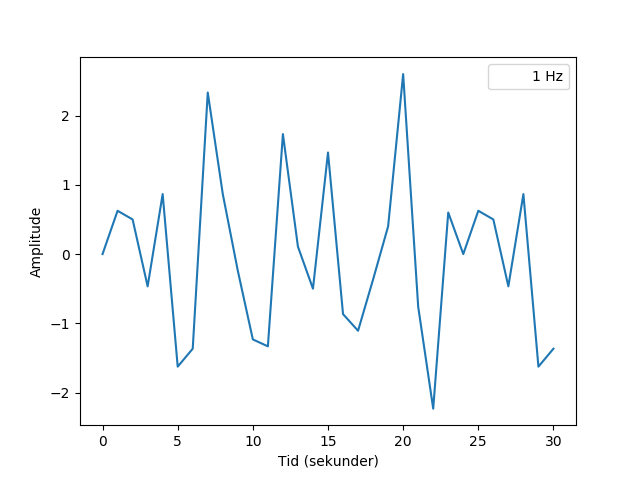
\includegraphics[width=\textwidth]{figures/signal_1hz.png}
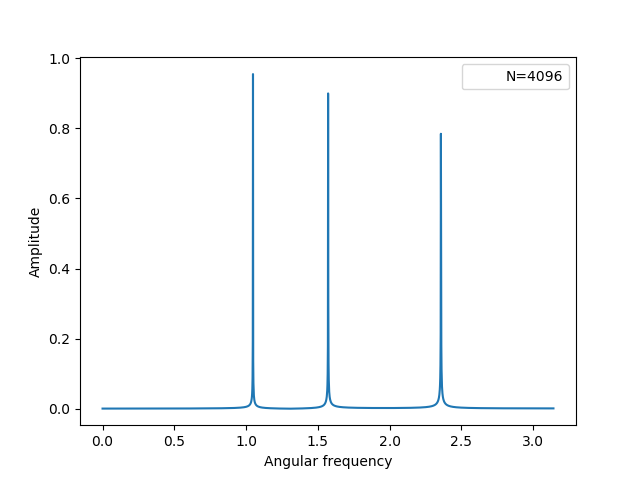
\includegraphics[width=\textwidth]{figures/frekvensanalyse/1hz_freq2}
\end{minipage}
\begin{minipage}{0.49\textwidth}
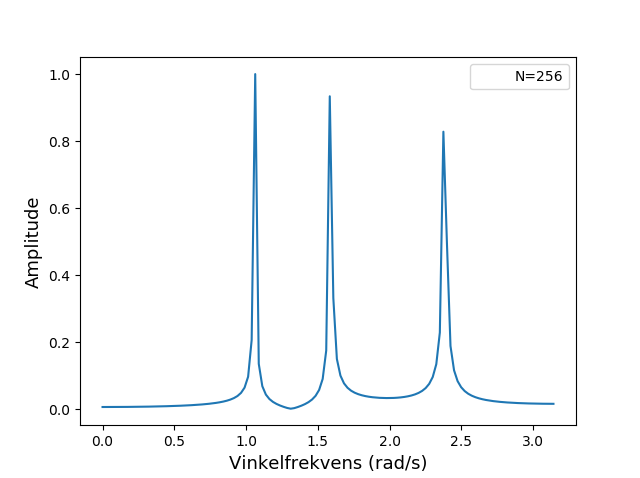
\includegraphics[width=\textwidth]{figures/frekvensanalyse/1hz_freq1.png}
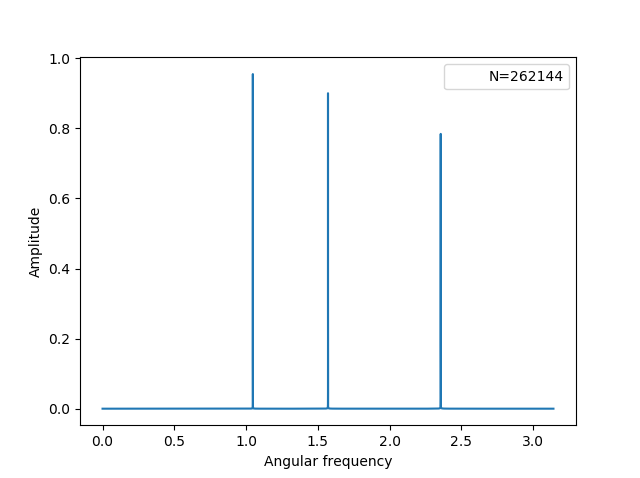
\includegraphics[width=\textwidth]{figures/frekvensanalyse/1hz_freq3.png}
\end{minipage}
\caption{Plot af signal samplet ved $f_s=1$ Hz i tidsdomænet og plot af de tilhørende frekvensdomæner for antal af samples $N = 2^8, 2^{12}, 2^{18}$.}
\label{fig:1}
\end{figure}

På figur \ref{fig:1} ses signalet ligeledes i tids- og frekvensdomænet samplet med $f_s=32$ Hz og med $N=2^8, 2^{12}, 2^{18}$ samples.

\begin{figure}[H]
\begin{minipage}{0.49\textwidth}
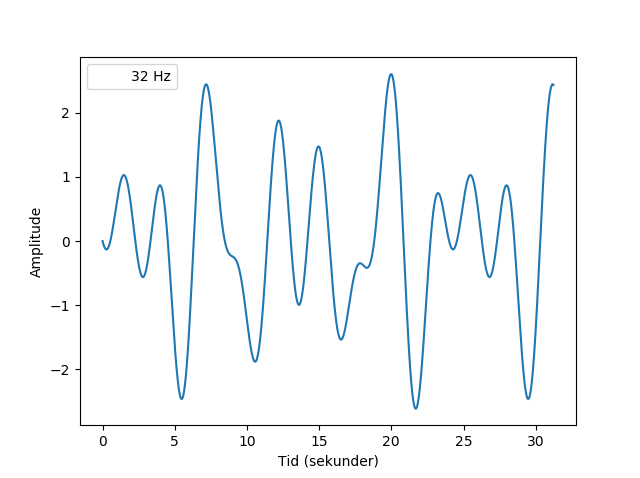
\includegraphics[width=\textwidth]{figures/signal_32hz.png}
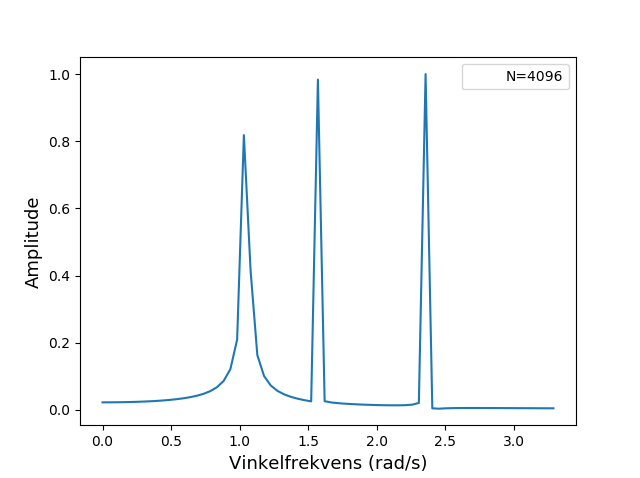
\includegraphics[width=\textwidth]{figures/frekvensanalyse/32hz_freq2}
\end{minipage}
\begin{minipage}{0.49\textwidth}
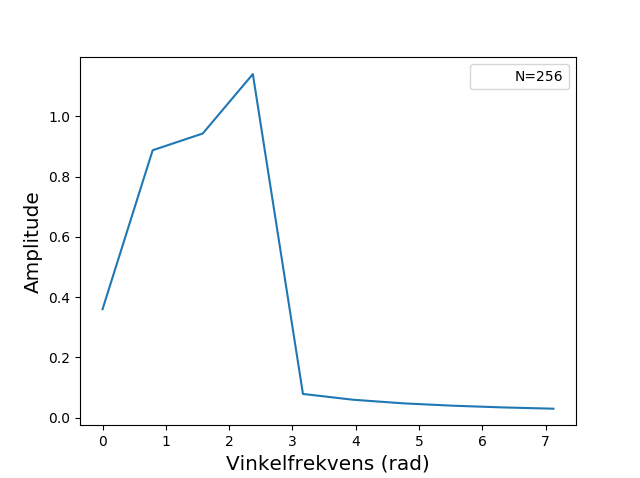
\includegraphics[width=\textwidth]{figures/frekvensanalyse/32hz_freq1.png}
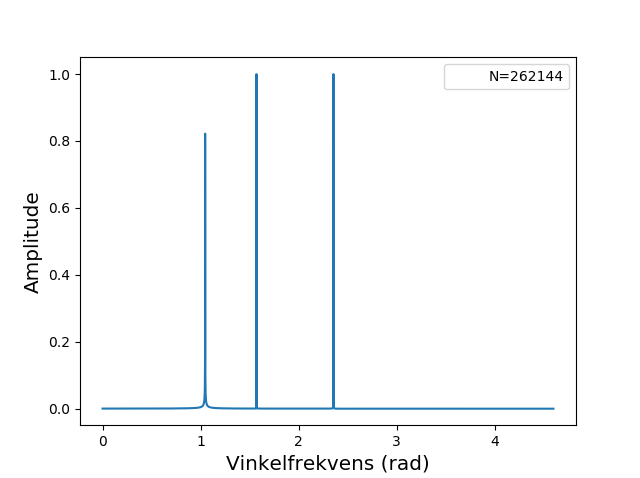
\includegraphics[width=\textwidth]{figures/frekvensanalyse/32hz_freq3.png}
\end{minipage}
\caption{Plot af signal samplet ved $f_s=32$ Hz i tidsdomænet og plot af udsnit af de tilhørende frekvensdomæner for antal af samples $N=2^8, 2^{12}, 2^{18}$.}
\label{fig:2}
\end{figure}

\section{Diskussion}
Det ses tydeligt på tidsdomænerne i figur \ref{fig:1} og figur \ref{fig:2}, at opløsningen af signalet i tid afhænger af $f_s$ og bliver bedre som $f_s$ stiger. Dette stemmer overens med \eqref{eq:tidsoploesning}.
\\ \\
Det ses ligeledes tydeligt, at opløsningen i frekvensdomænet afhænger af $N$ og bliver bedre som $N$ stiger. Det er ydermere bemærkelsesværdigt, at øgning af $f_s$ giver ringere opløsning i frekvensdomænet som set i andet plot i figur \ref{fig:2}. Disse observationer stemmer ligeledes overens med \eqref{eq:tidsoploesning}.
\\ \\
Det ses i figur \ref{fig:1} og \ref{fig:2}, at amplituderne for de tre frekvenser, som signalet indeholder, ikke er lige store, selvom signalet tydeligvis er konstrueret således. Det ses også på figur \ref{fig:1} og figur \ref{fig:2}, at amplituderne varierer som $f_s$ varierer, men ikke som $N$ varierer. Dette skyldes spektral lækage, og er ikke et problem for rekonstruktion af signalet, da energien blot er distribueret rundt om den frekvens, som den bør forefindes ved, således amplituden bliver 1.

\section{Delkonklusion}
Frekvensanalysen af signalet afslørede tydeligt de tre frekvenser, som optræder i signalet, og det blev vist, hvordan opløsningen af signalet i tid og frekvens afhænger af $f_s$ og $N$ - bedre opløsning i tid betyder generelt ringere opløsning i frekvens og omvendt. At lade $N$ være arbitrært stor er ikke en mulighed, da den beregningsmæssige kompleksitet afhænger af $N$ og der ikke haves uendelig regnekraft. På baggrund af disse overvejelser skal der træffes en beslutning om fastlæggelsen af $f_s$ og $N$.
















